\underline{\textit{Microsoft Copilot Output \#1: State Space}}\\

\noindent \textbf{Q:} so i have a walker rollator with 4 ultrasonic sensors returning distance (2 front facing, 2 laterally facing), 1 lidar sensor returning distance (front facing), an IMU providing acceleration x,y,z and angles x,y,z. there are haptic motors which buzz if range readings are low and also braking for the same purpose. i want to make a state space representation taking into account a Yaw angle steering command and also a motor spin speed command based on the appropriate inputs

\noindent \textbf{A:} \\
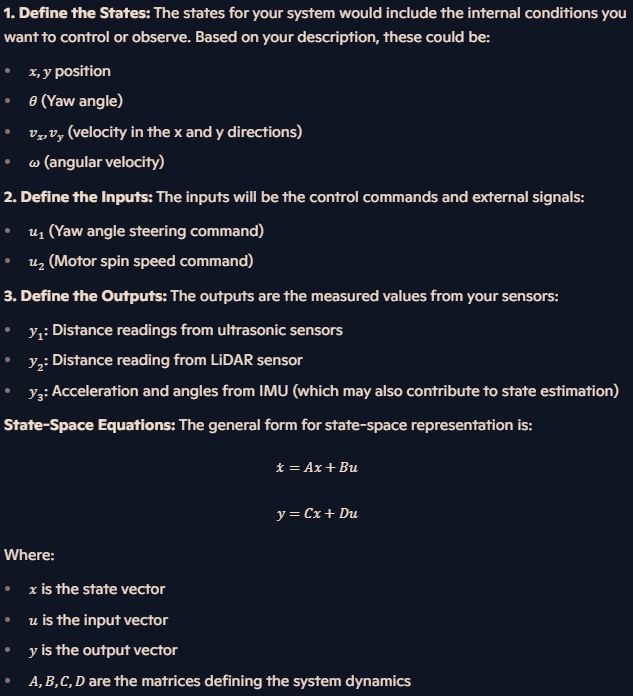
\includegraphics[width=0.535\textwidth]{./Images/copilot-ssr.JPG}
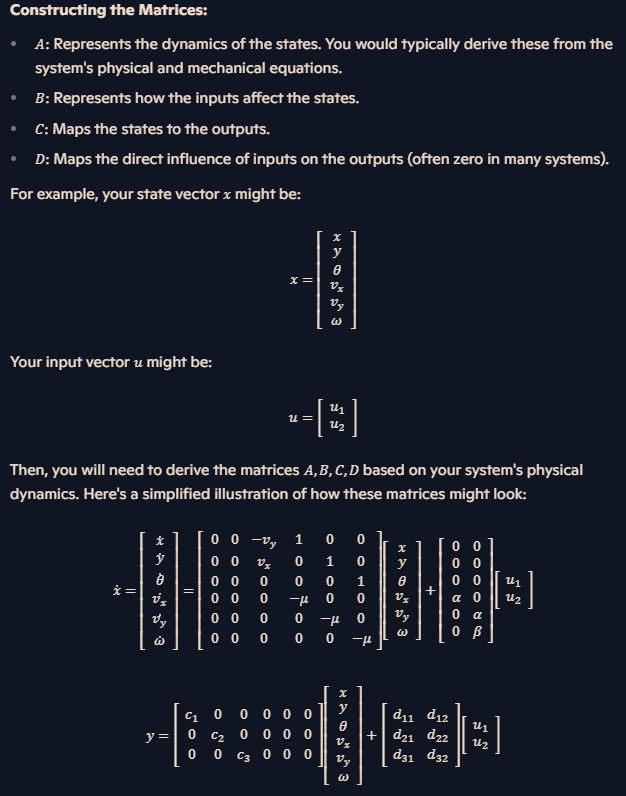
\includegraphics[width=0.465\textwidth]{./Images/copilot-ssr2.JPG}

\underline{\textit{Microsoft Copilot Output \#2: FCC}}\\

\noindent \textbf{Q:} fcc acronym

\noindent \textbf{A:} \\

\includegraphics[width=0.535\textwidth]{./Images/fcc_ai.png}
